% !TeX root = ../../msc-thesis.tex
\documentclass[../../msc-thesis.tex]{subfiles}

\begin{document}

\section{The CO\texorpdfstring{\textsubscript{2}}{\space} Compression and 
Purification Unit (CPU)}

The first case-study to be used as a test-bed in \mtc consists in a 
\co compression and purification unit that uses phase 
separation method to obtain purified \co from oxy-fuel 
combustion. This process is one of the several that exist in the industry 
that are capable of reducing the greenhouse effect on climate 
change \cite{Jin2015}. The process and its simulation are based on the work 
of \textcite{Liu2019}. In addition, their unit is based on the prototype 
proposed by the International Agency Greenhouse Gas (IEAGHG) R{\&}D 
program study \cite{Dillon2005}.
\nomenclature[A]{IEAGHG}{International Agency Greenhouse Gas}

The process is depicted in \autoref{fig:cpuflowsheet}. Flue gas is compressed 
by a three-stage after-cooled compressor before being sent to the cold 
box, where two multi-stream heat exchangers (E1 and E2) and two separators 
(F1 and F2) take place. In the base case from \textcite{Liu2019}, the flue gas 
is first cooled to $-24.51\celsius$ and sent to to F1, with its bottom 
stream being the first product of the process. Afterwards, The top stream 
from F1 is sent to the second multi-stream heat-exchanger (E2) being cooled 
to $-54.69\celsius$ before going to separator F2. The bottom stream 
from this separator consists in the second product of the process, and the 
top stream from F2 is discarded as vent. Both \co product streams and the 
vent gas are reheated on both multi-stream heat exchangers. The \co product 
streams are mixed and become ready for storage. The reader can consult 
\textcite{Jin2015} and \textcite{Liu2019} for more information about the 
simulation (i.e.: Raw flue gas conditions, detailed stream and equipment 
conditions, etc).

\begin{figure}[htb]
    \caption{CPU process flowsheet}
    \centering
    \makebox[1.0\textwidth]{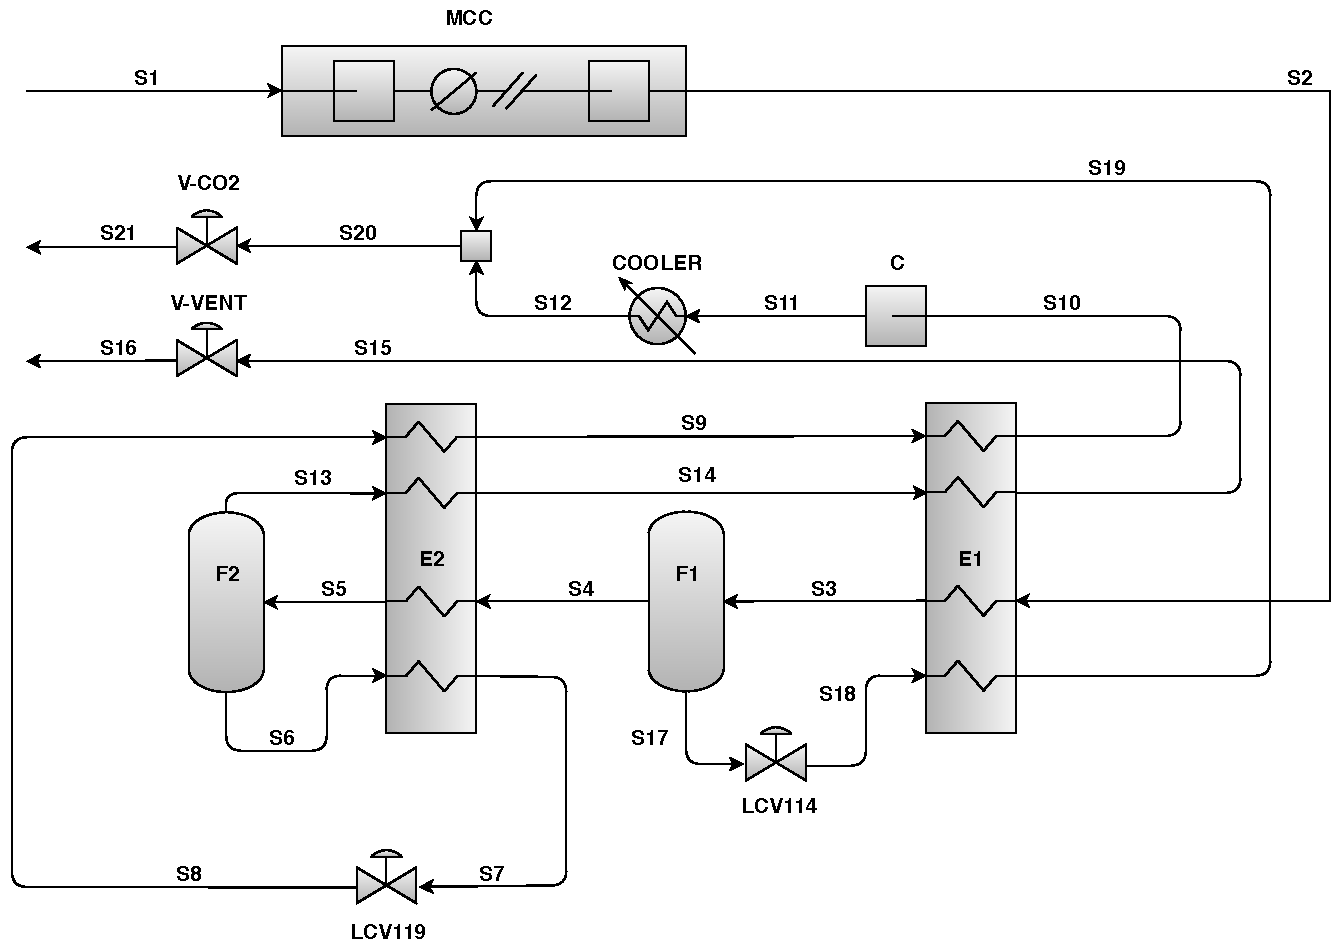
\includegraphics[width=1.0\textwidth]
    {CPUflowsheet.pdf}}
    \fonte{Author}
    \label{fig:cpuflowsheet}
\end{figure}

From \textcite{Liu2019}, the authors of this paper have selected the objective 
function described in \autoref{eq:eq1}, that consists in the specific energy 
consumption, defined as the ratio of energy used in both compressors 
(MCC and C) to total \co flow rate produced. Therefore:

\begin{equation}
    J=\frac{W_{\mathrm{MCC}}+W_{\mathrm{C}}}{F_{\mathrm{CO}_{2}}}
    \label{eq:eq1}
\end{equation}

The units of specific energy consumption of the objective function are 
$kWh/{tCO\textsubscript{2}}$.

Regarding the CPU process constraints, from \textcite{Jin2015},
\textcite{Liu2019} and \textcite{Dillon2005}, the following apply:

\begin{itemize}
    \item C-1: \co recovery rate $\geq 90 \%$
    \item C-2: \co purity on product stream  $\geq 96 \%$
    \item C-3: Temperature of F2 bottom stream $>-56.6\celsius$
\end{itemize}

C-1 aims to meet the environmental requirements \cite{Liu2019} and reduce 
\co atmospheric emissions \cite{Toftegaard2010, Buhre2005}. 
C-2 is a result of the demand of \co storage and transportation 
\cite{Liu2019}. In addition, according to \textcite{Posch2012}, the purity 
addressed in this constraint would realize acceptable energy consumption. 
Lastly, C-3 exists to avoid \co solidification in the pipeline, since the 
value of C-3 corresponds to the \co three-phase freezing point 
\cite{Posch2012, Koohestanian2017}.

As stated by \textcite{Liu2019}, the main disturbances in the CPU process are:

\begin{itemize}
    \item D-1: Flue gas flow rate
    \item D-2: \co concentration in the flue gas
\end{itemize}

D-1 and D-2 are a result of the oxy-fuel combustion boiler island 
\cite{Liu2019}, given the variation of the boiler operation. Load changes 
in the boiler island and variations of the combustion conditions can 
generate D-1 and D-2, as also stated by \textcite{Liu2019}. It is considered 
a $\pm 5 \%$ disturbance amplitude for \co feed composition and flue gas 
flow rate of the base-case, similarly as \textcite{Jin2015} and 
\textcite{Liu2019}.

The number of degrees of freedom for the CPU process is 4 \cite{Jin2015, 
Liu2019} for Mode I (Given feed). For the sake of simplicity and without 
loss of generality, the same DOFs from \textcite{Jin2015} were used here:
\nomenclature[A]{DOF}{Degree of Freedom}

\begin{enumerate}
    \item MCC outlet pressure (bar)
    \item MCC outlet temperature $(\celsius)$
    \item F1 temperature $(\celsius)$
    \item F2 temperature $(\celsius)$
\end{enumerate}

Using this information and based on the review of control configurations 
for \co CPU process \cite{Liu2019}, the CV candidates in 
\autoref{tab:cvcandidateslist} that were considered in this case 
study are listed.

\begin{table}[htb]
    \centering
    \caption{CV Candidates for $CO_{2}$ CPU process.}
    \begin{tabular}{l l}
    \hline
    \textbf{Variable} (alias used in \mtc) & \textbf{Description} \\ \hline
        mccp/mccpout & Compressor outlet pressure (bar) \\
        mcct/mcctout & Compressor outlet temperature $(\celsius)$ \\
        f1t/f1tout  & F1 temperature $(\celsius)$\\
        f2t/f2tout  & F2 temperature $(\celsius)$  \\
        s8t         & S8 stream temperature $(\celsius)$ \\
        fco2out     & $CO_{2}$ product flowrate $(t/h)$\\
        xco2out     & $CO_{2}$ product molar fraction \\
        co2rr       & $CO_{2}$ recovery rate \\
    \hline
    \end{tabular}
    \label{tab:cvcandidateslist}
\end{table}


With 4 degrees of freedom and 8 CV candidates, there are 
(\autoref{eq:cpupossible})

\begin{equation}
    \binom{8!}{4!} = \frac{8!}{4!\times(8-4)!} = 70
    \label{eq:cpupossible}
\end{equation}

possible control structures for a single measurement policy (excluding the 
possible ways of controlling the regulatory layer and the possibility of 
using linear combinations of measurements). Therefore, the manual evaluation 
of all possibilites is impracticable and also would need the usage of 
different software environments. This tedious evaluation, however, can be 
mitigated by \mtc.

With the problem defined and the possible CV candidates being listed, 
it is possible to start to use the capabilities of \mtc in order to aid 
the search for a \soc structure for this case-study. Initially, it is 
necessary to seek for the variables of the process simulator (Aspen Plus) 
using the COM interface between the \mtc software and the process simulator. 

\Cref{fig:mainscreen,,fig:loadvar} illustrate the process of selecting a 
*.bkp file, selecting the relevant variables, and adding alias to them.

\begin{figure}[htb]
    \caption{\mtc main screen with CPU process simulation file loaded.}
    \centering
    \makebox[1.0\textwidth]{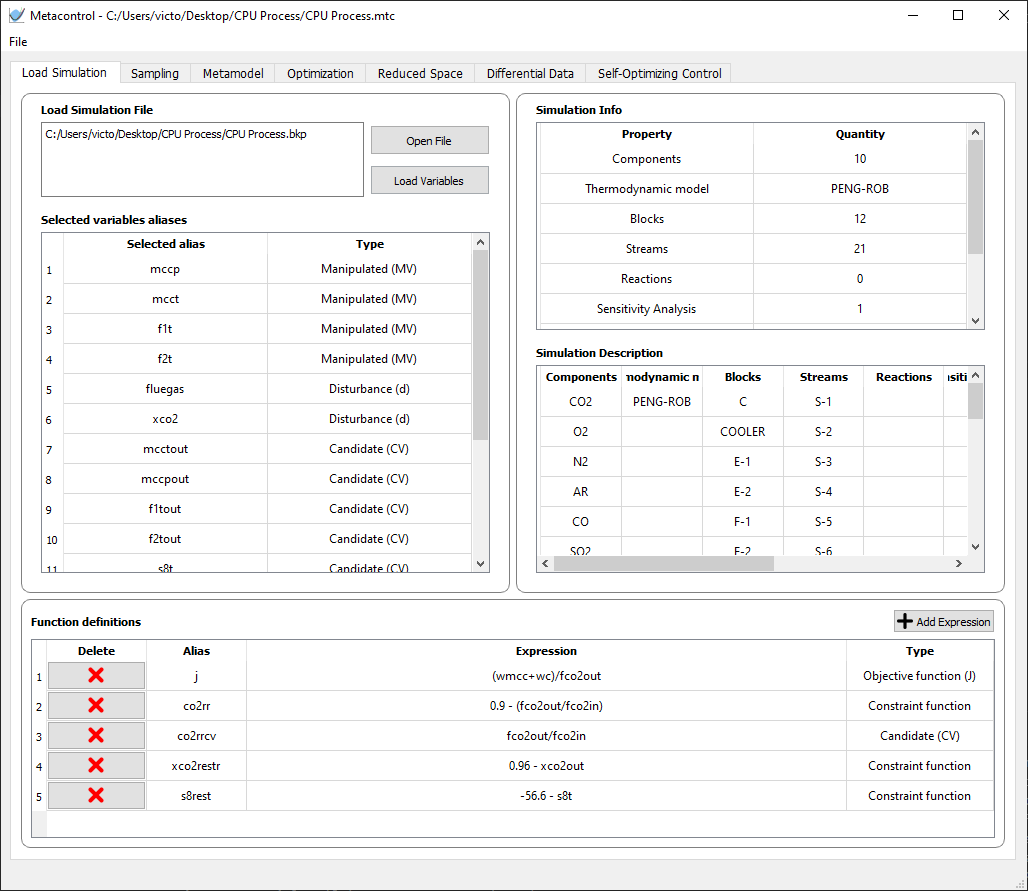
\includegraphics[width=1.0\textwidth]
    {mainscreen.PNG}}
    \label{fig:mainscreen}
    \autfont
\end{figure}

\begin{figure}[htb]
    \centering
    \caption{Loading variables for the CPU from Aspen Plus simulation and 
    adding alias to them. At the top right corner of this screen, the user is 
    able to select the option to reveal the GUI from Aspen Plus. This features 
    allows the user to inspect inside the process simulator interface to 
    remember any stream or block names. This can be helpful when one is 
    selecting the variables using the COM technology and there are several 
    unit operations blocks and streams, for instance. Another feature that 
    was implemented in order to ease the search of the variables, regards 
    the description of each variable: Hovering the mouse over a COM variable 
    will show its description, extracted directly from the process simulator.}
    \makebox[1.0\textwidth]{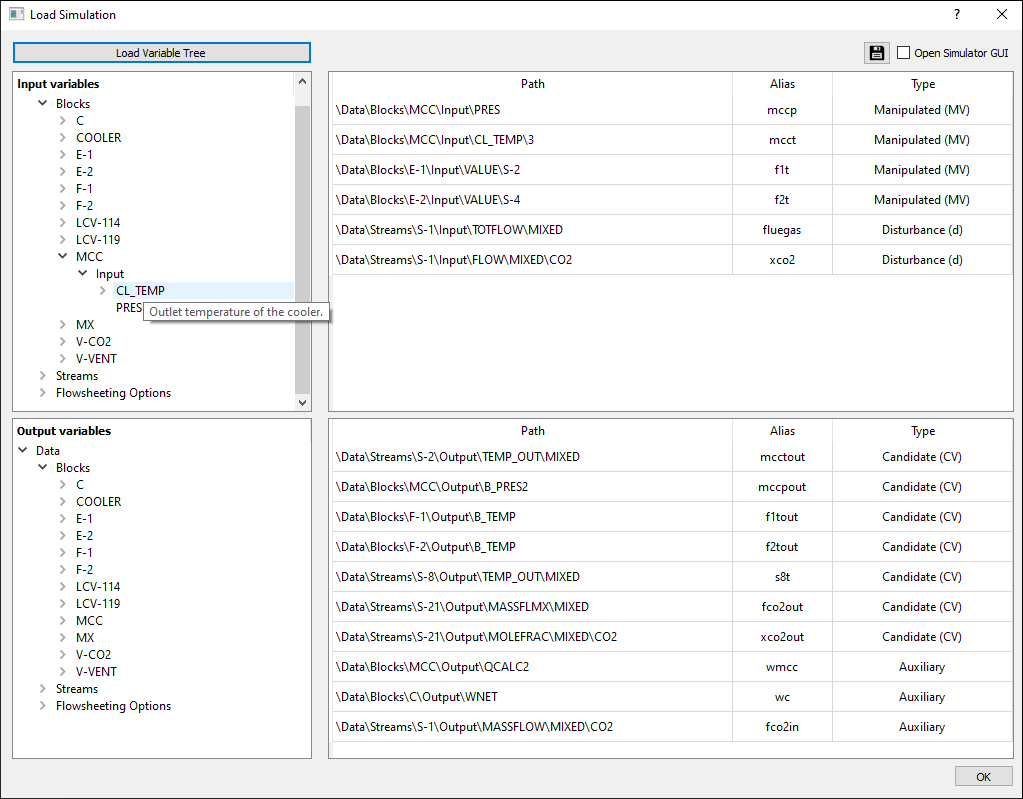
\includegraphics[width=1.0\textwidth]{loadvar.PNG}}
    \label{fig:loadvar}
    \autfont
\end{figure}

From \autoref{fig:mainscreen} the user can see that \mtc shows on its 
main screen some relevant information: Block names, flowsheet operations 
(i.e.: Optimizations, sensitivities, calculators), the components selected 
in the process simulated and the thermodynamic package used. These are 
enumerated on ``Simulation Info'' panel and the name of each object is 
present on ``Simulation Description'' panel.

After selecting the relevant variables (Decision variables and process 
measurements) the user can go back to the main screen, where expressions 
can be created. This functionality aims to give freedom for the user to 
build expressions based on variables from the process simulator, such as: 
Objective functions, CV candidates or constraints. \autoref{fig:expreval} 
shows the specific power consumption, the \co recovery rate expressions 
being built, based on the auxiliary variables selected on 
\autoref{fig:loadvar}.

\begin{figure}[htb]
    \centering
    \caption{Creating expressions for specific power consumption (objective 
    function), \co recovery rate and S8 Temperature 
    (constraint functions/CV candidates).}
    \label{fig:expreval}
    \makebox[1.0\textwidth]{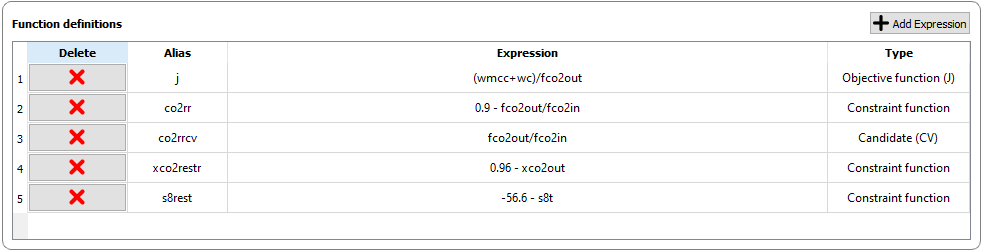
\includegraphics[width=1.0\textwidth]
    {expressionval.PNG}}
\end{figure}

With the procedure aforementioned being completed, the user can generate 
the design of experiments (DOE) in order to build \kriging responses of the 
objective function, CV candidates and process constraints. The ranges for 
each decision variable are taken from \textcite{Jin2015} (Table 3 from their
paper), and this step is illustrated in \Crefrange{fig:lhs1}{fig:lhs3}.

\nomenclature[A]{DOE}{Design Of Experiments}
\nomenclature[A]{LHS}{Latin Hypercube Sampling}

\begin{figure}[htb]
    \centering
    \caption{\mtc ``Sampling panel''. The user can perform the 
    sampling using the process simulator or import a .CSV file.}
    \label{fig:lhs1}
    \makebox[1.0\textwidth]{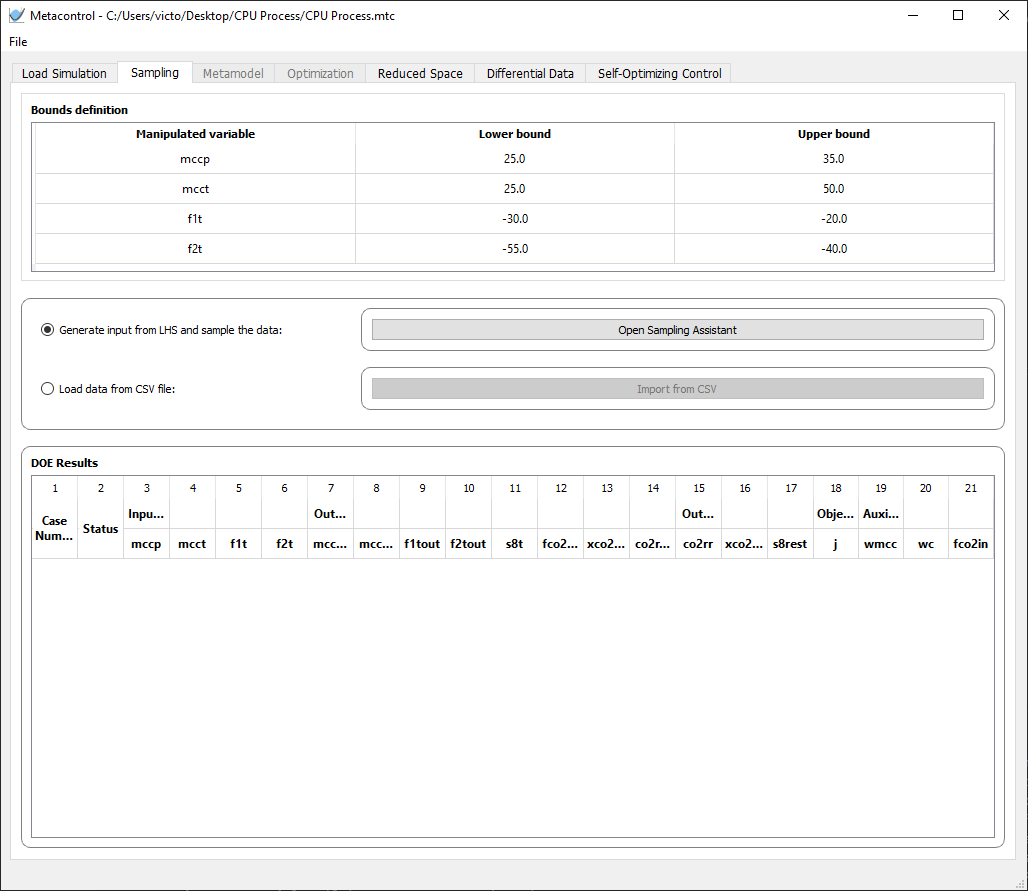
\includegraphics[width=1.0\textwidth]{lhs_1.PNG}}
\end{figure}

\begin{figure}[htb]
    \centering
    \caption{\mtc Sampling assistant. The limits for the 
    decision variables used in the CPU process are the same from 
    \textcite{Jin2015} and \textcite{Liu2019}}
    \label{fig:lhs2}
    \makebox[1.0\textwidth]{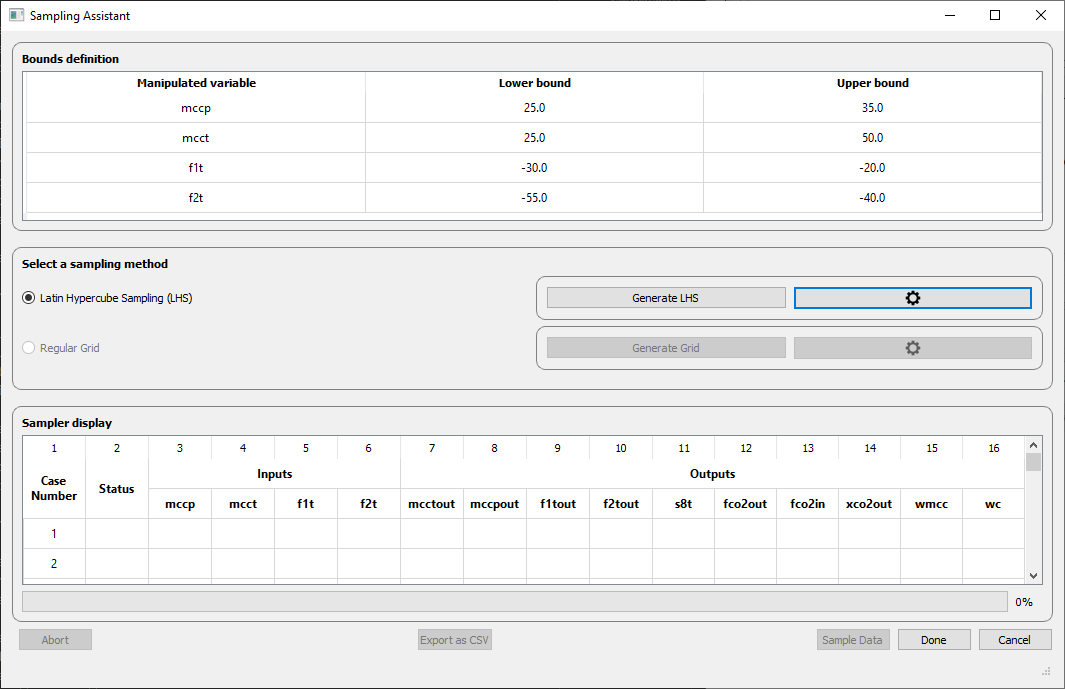
\includegraphics[width=1.0\textwidth]{lhs_2.PNG}}
\end{figure}

\begin{figure}[htb]
    \centering
    \caption{\mtc Latin Hypercube Sampling settings. 80 
    samples were generated and 5 iterations were performed in order to try 
    to maximize the minimum distance between the points (\textit{maxmin} 
    criterion). The user can also add the vertices of the design of 
    experiments.}
    \label{fig:lhs3}
    \makebox[1.0\textwidth]{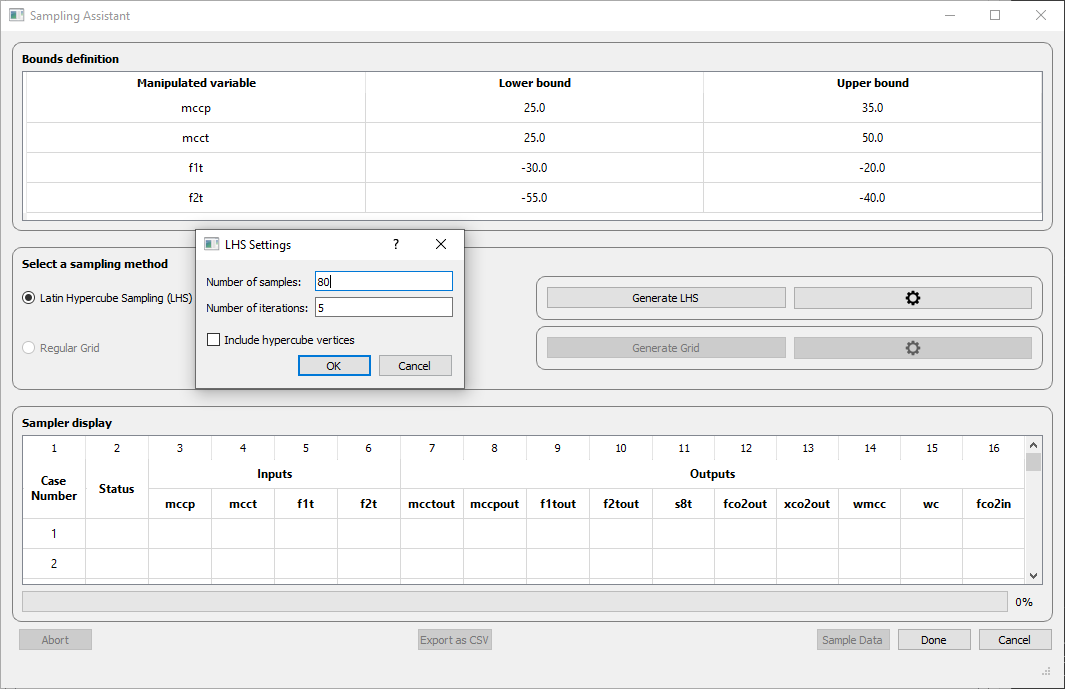
\includegraphics[width=1.0\textwidth]{lhs_3.PNG}}
\end{figure}

\autoref{fig:lhs4} shows the sampling process running. After running all 
cases, the user can inspect the results of the design of experiments, as 
can be seen in \autoref{fig:lhs5}.
	
\begin{figure}[htb]
    \centering
    \caption{\mtc Sampling for the CPU process.}
    \label{fig:lhs4}
    \makebox[1.0\textwidth]{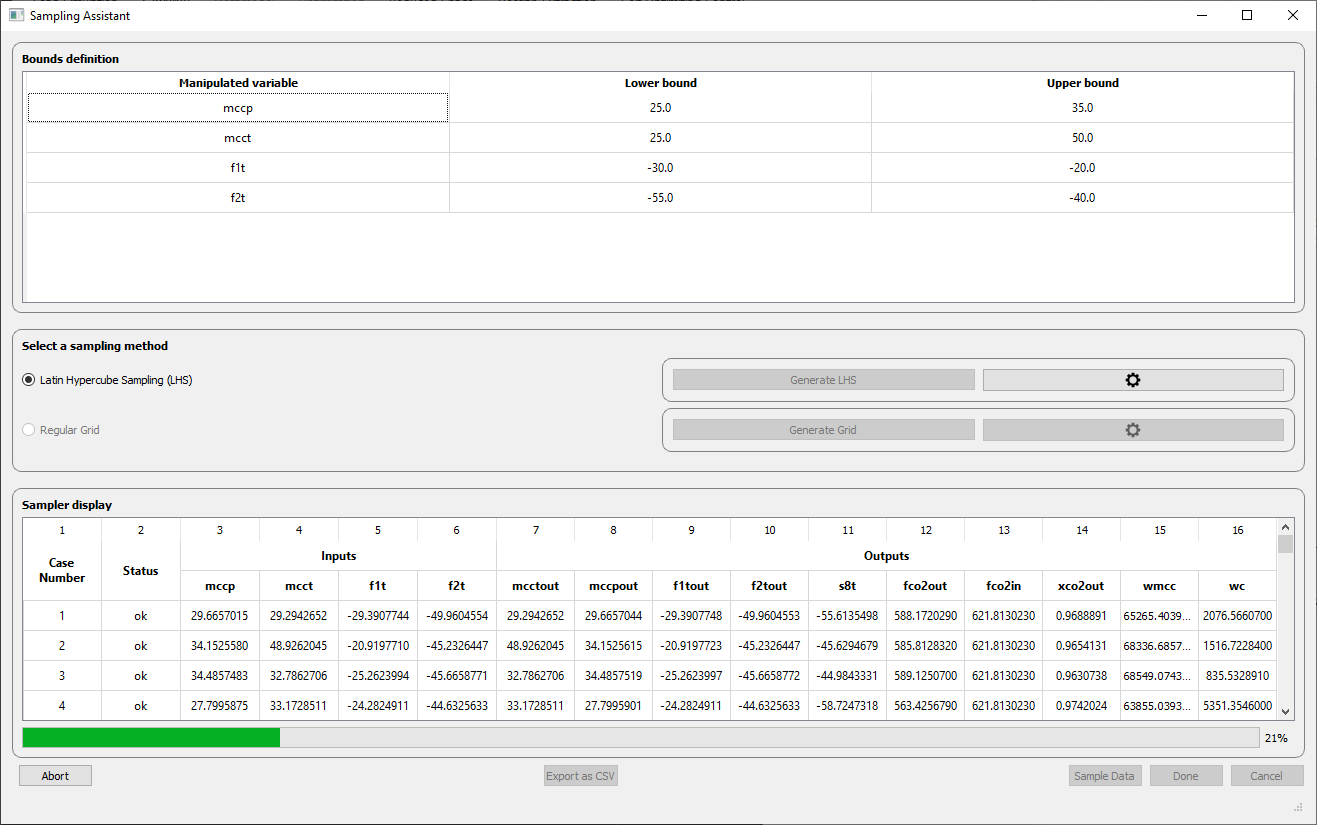
\includegraphics[width=1.0\textwidth]{lhs_4.PNG}}
\end{figure}


\begin{figure}[htb]
    \centering
    \caption{Sampling results, where the user can inspect convergence 
    status and the values of the selected variables for each case.}
    \label{fig:lhs5}
    \makebox[1.0\textwidth]{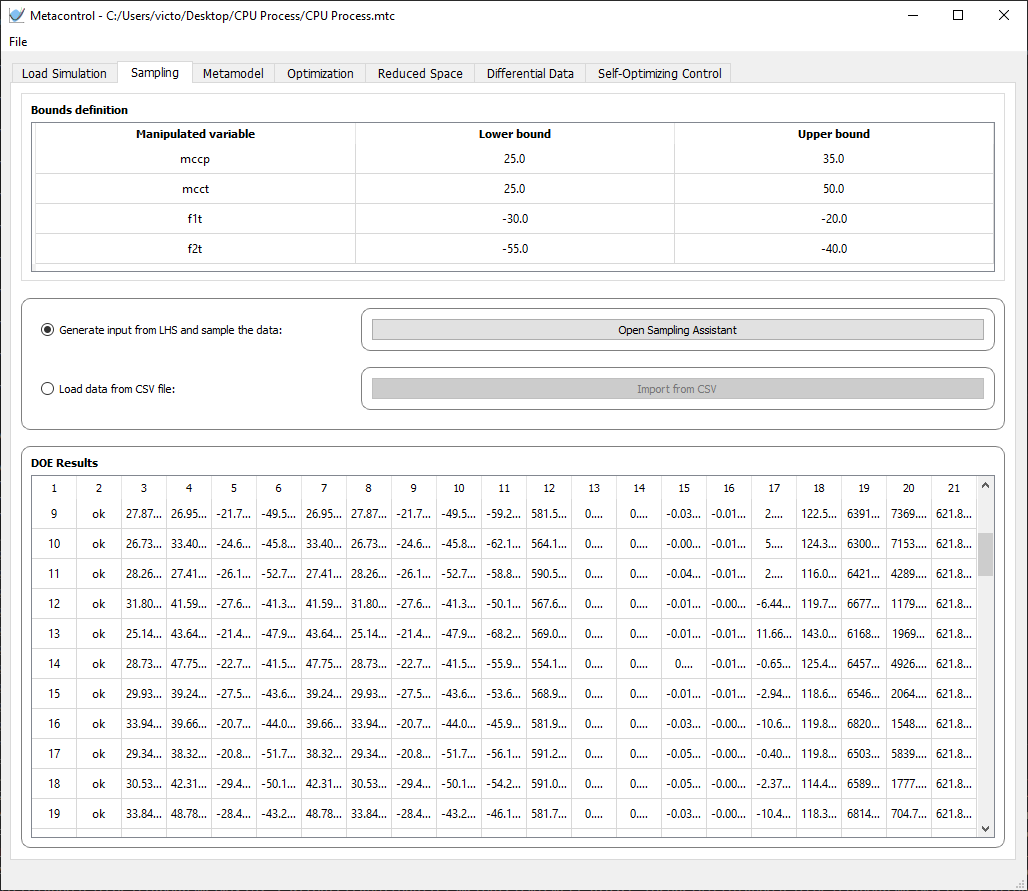
\includegraphics[width=1.0\textwidth]{lhs_5.PNG}}
\end{figure}

With the results of the sampling procedure, the user can go to the 
``Metamodel'' Panel, and select which variables will have \kriging responses 
built, the bounds for the \kriging hyperparameters optimization, and the 
regression and correlation models to be used. This procedure can be depicted 
in \autoref{fig:krigingresults}.

The user can also choose which type of validation is going to be performed:
\textit{Hold-out} or \textit{K-fold} validation. It is important to point 
out that this first metamodel generation is performed only to give a 
quick view of the initial sampling. In other words, to check if the initial 
sampling is acceptable to be refined by the implementation of the algorithm 
proposed by \textcite{Caballero2008} that is bundled in \mtc. In addition, 
if the user chooses \textit{Hold-out} validation, it is possible to view 
the graphical results (fitness of training set to the metamodel) of each 
\kriging interpolator generated, as can be seen in \autoref{fig:plotkr}.

In \autoref{fig:krigingresults}, the reader can also inspect under the
panel ``Validation metrics'', several metrics are used to evaluate reduced 
models performance, such as: Mean squared error (MSE), Root mean squared 
error (RMSE), Mean absolute error (MAE), $R^{2}$ linear coefficient,
Explained variance (EV), the Sample mean and also its standard deviation.

\begin{figure}[htb]
    \centering
    \caption{\kriging configuration and validation metrics results.}
    \label{fig:krigingresults}
    \makebox[1.0\textwidth]{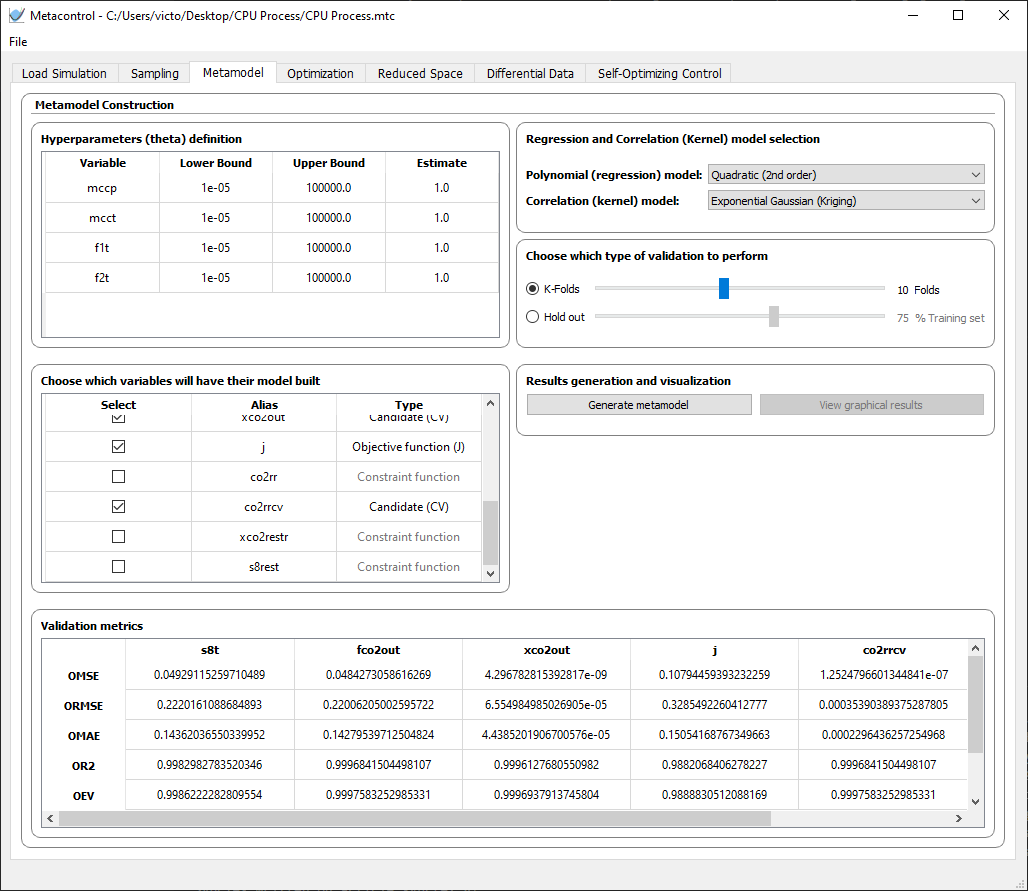
\includegraphics[width=1.0\textwidth]
    {krigingresults.PNG}}
\end{figure}

\begin{figure}[htb]
    \centering
    \caption{Fitness for each metamodel.}
    \label{fig:plotkr}
    \makebox[1.0\textwidth]{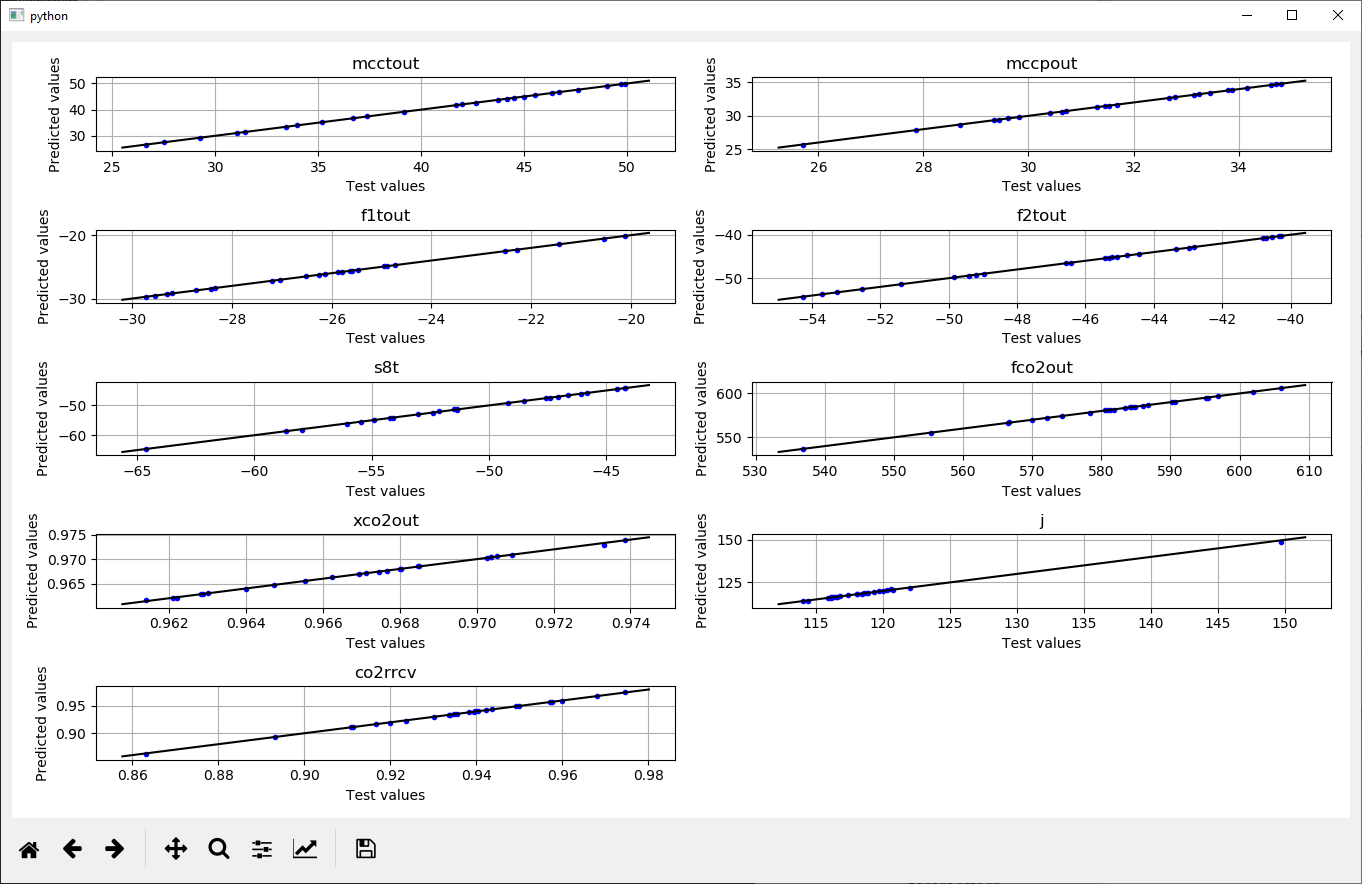
\includegraphics[width=1.0\textwidth]
    {graphical_results.PNG}}
\end{figure}

In order to try to improve the initial sampling for optimization purposes, 
we go to the ``Optimization'' tab where the refinement algorithm proposed by 
\textcite{Caballero2008} is implemented. \autoref{fig:caballeroscreen} 
shows the parameters that can be tuned in order to attempt to improve the 
\kriging interpolator using the automated refinement procedure, with further 
discussion and details regarding each parameter can be found on 
\textcite{caballero2008} and in the previous work from the author of this 
dissertation \cite{Alves2018}. In addition, NLP solvers parameters can 
also be changed in this screen. 

In \autoref{fig:caballeroscreen}, the user can see the final result of 
the refinement algorithm: on the ``Results'' panel, the final results for 
the decision variables, constraints expressions defined previously and the
objective function. In addition, a control panel showing the operations of
contraction and movement of the hyperspace performed by the algorithm 
(and how many iterations on each operation) can be inspected.  
\autoref{fig:caballerocmd} shows the control panel details of the procedure.

\begin{figure}[htb]
    \centering
    \caption{Refinement algorithm configuration and results screen.}
    \label{fig:caballeroscreen}
    \makebox[1.0\textwidth]{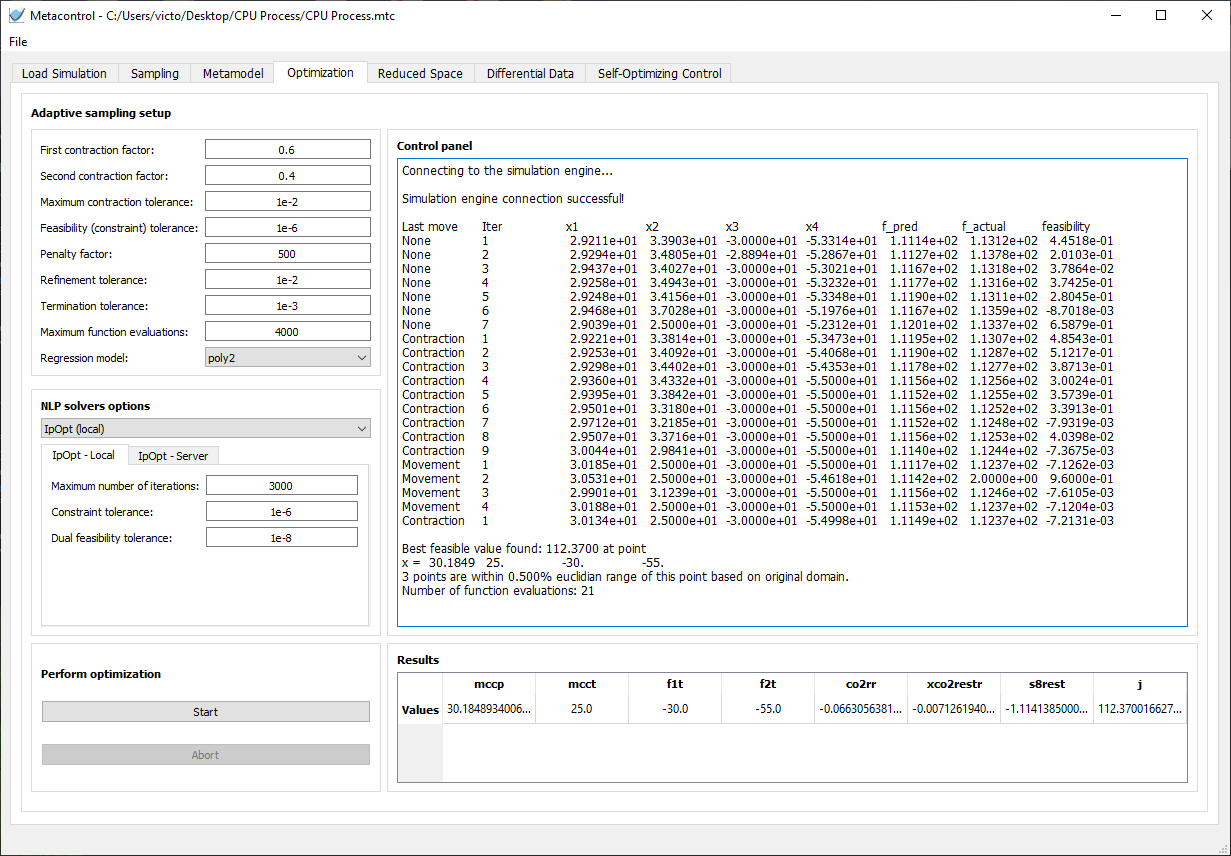
\includegraphics[width=1.0\textwidth]
    {caballeroscreen.PNG}}
\end{figure}

\begin{figure}[htb]
    \centering
    \caption{Refinement algorithm control panel output.}
    \label{fig:caballerocmd}
    \makebox[1.0\textwidth]{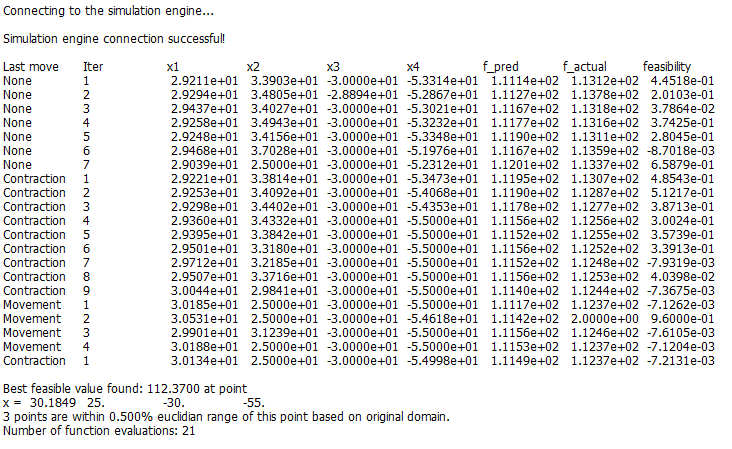
\includegraphics[width=1.0\textwidth]
    {caballerocmd.PNG}}
\end{figure}

Inspecting \Cref{fig:caballeroscreen,,fig:caballerocmd}, it is clear that
the optimal operating point found is

\begin{itemize}
    \item MCC outlet pressure (bar) = 30.1849
    \item MCC outlet temperature = 25 $\celsius$
    \item F1  temperature = -30 $\celsius$
    \item F2  temperature = -55$\celsius$
\end{itemize}

That indicates three active constraints that have to be controlled. 
Regarding stream S8 temperature, \co product purity and recovery rate,
these were inactive constraints. Therefore, the reduced space problem has one
degree of freedom left for \soc.

In order to prove the effectiveness of the proposed software and the 
procedures and algorithms used, an optimization using the process
simulator (Aspen Plus) SQP implementation (an optimization block) was 
performed, and the results can be found in 
\Cref{tab:optcomparison1,,tab:optcomparison2}, compared with the results 
found by \mtc. They identical, quantitatively and 
qualitatively (the active constraints found in both approaches). The 
constraints in \mtc are written internally in the form g(x)$\leq 0$, and 
showed in the GUI in the same way, due to NLP solvers and refinement 
algorithm syntaxes.

\begin{table}[htb]
    \centering
    \caption{Optimization runs: \textit{Aspen Plus vs Metacontrol} - Decision
    variables and objective function - CPU Process}
    \resizebox{\textwidth}{!}{
    \begin{tabular}{c c c c c c c}

        \hline
         & Objective function J (kWh/t\co) & MCC Pressure (bar) & 
        MCC outlet temperature ($\celsius$) & F1 temperature ($\celsius$) & 
        F2 temperature ($\celsius$) \\
        \hline
        Aspen Plus & 112.3690 & 30.0316 & 25 & -30 &-55 \\
        \mtc & 112.3691 & 30.1849 & 25 & -30 & -55\\
        \hline
    \end{tabular}
    }
    \label{tab:optcomparison1}
\end{table}

\begin{table}[htb]
    \centering
    \caption{Optimization runs: \textit{Aspen Plus vs Metacontrol} - Process
    constraints - CPU Process}
    \resizebox{\textwidth}{!}{
    \begin{tabular}{c c c c c c c}

        \hline
         & Stream S8 temperature $\celsius$ & 
         \co molar fraction & 
         \co recovery rate \\
        \hline
        Aspen Plus & -55.8201 & 0.9674 & 0.9658 \\
        \mtc & -55.4859 & 0.9666 & 0.9671\\
        \hline
    \end{tabular}
    }
    \label{tab:optcomparison2}
\end{table}

After determining the nominal optimal operating point, the active
constraints must be implemented in the simulation file externally using the 
process simulator (Using design specifications for instance) and go back to 
\mtc, in order to generate the reduced space \kriging metamodel, seeking the 
obtainment of differential data (e.g.: the gradients $G_{y}$,$G_{y}^{d}$, 
and the hessians $J_{uu}$ and $J_{ud}$). The reduced space problem can be 
sampled using the process simulator linked with \mtc directly, or importing 
a *.csv file. Both options mentioned are similar to the initial sampling 
procedure. 

Over the tab ``Differential data'', the user is capable of checking which 
variables are active constraints (either decision variables or nonlinear 
constraints), inserting the values for the optimal operating point found on 
the previous step (refined surrogate optimization), and the value for the 
nominal disturbances. If the user sample the reduced space problem using 
the *.bkp, he must also input the range for the remaining decision variables 
to be sampled and for the disturbances. The range for the remaining degrees 
of freedom and for the disturbances are suggested to be a small percentage 
of the nominal values ($\pm 0.5\%$, for instance) in order to train a surrogate 
model accurate enough at the optimal region, guaranteeing robust high-order 
data (gradients and hessians) obtainment, as suggested previously in 
\textcite{Alves2018}.

In the CPU process, the MCC operating pressure, MCC temperature, F1 
temperature and F1 temperature are active constraints as mentioned previously. 
Therefore, they should be marked as ``active'' under the ``Variable activity'' 
panel, as shown in \autoref{fig:variableactivity}.

\begin{figure}[htb]
	\centering
    \caption{``Variable activity'' panel, where the user is capable of 
    highlighting which variables are active constraints and inputting values 
    for them. If an active constraint is a nonlinear constraint, the user 
    must pair this variable with a decision variable (MV) to consume a 
    degree of freedom.}
	\label{fig:variableactivity}
    \makebox[1.0\textwidth]{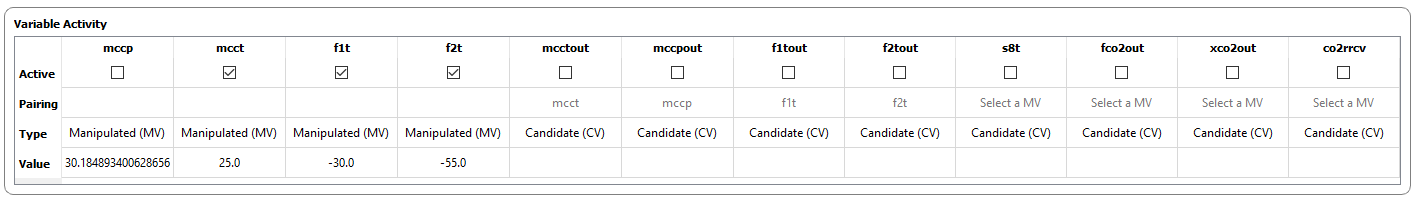
\includegraphics[width=1.0\textwidth]
    {variableactivity.PNG}}
\end{figure}

Since in the initial sampling the process simulator was directly linked with 
\mtc, in \autoref{fig:variableactivity} under the ``Data source'' panel a 
.*csv file was imported, originated from a sensitivity analysis run done in 
a *.bkp file of the reduced space problem for the CPU process, in order to 
show this supplementary feature of \mtc. This is illustrated in 
\Cref{fig:csvload,,fig:csvassociate}.

\begin{figure}[htb]
	\centering
	\caption{Loading a *.csv file in containing design of experiments data in 
    \mtc: if the user chooses this option, he must provide a file containing 
    all variables selected from the first step (``Load variables'' under 
    ``Load simulation'' tab). the convergence flag is used as a header to
	map the *.csv, and the software asks the user to select it.}
	\label{fig:csvload}
	\makebox[1\textwidth]{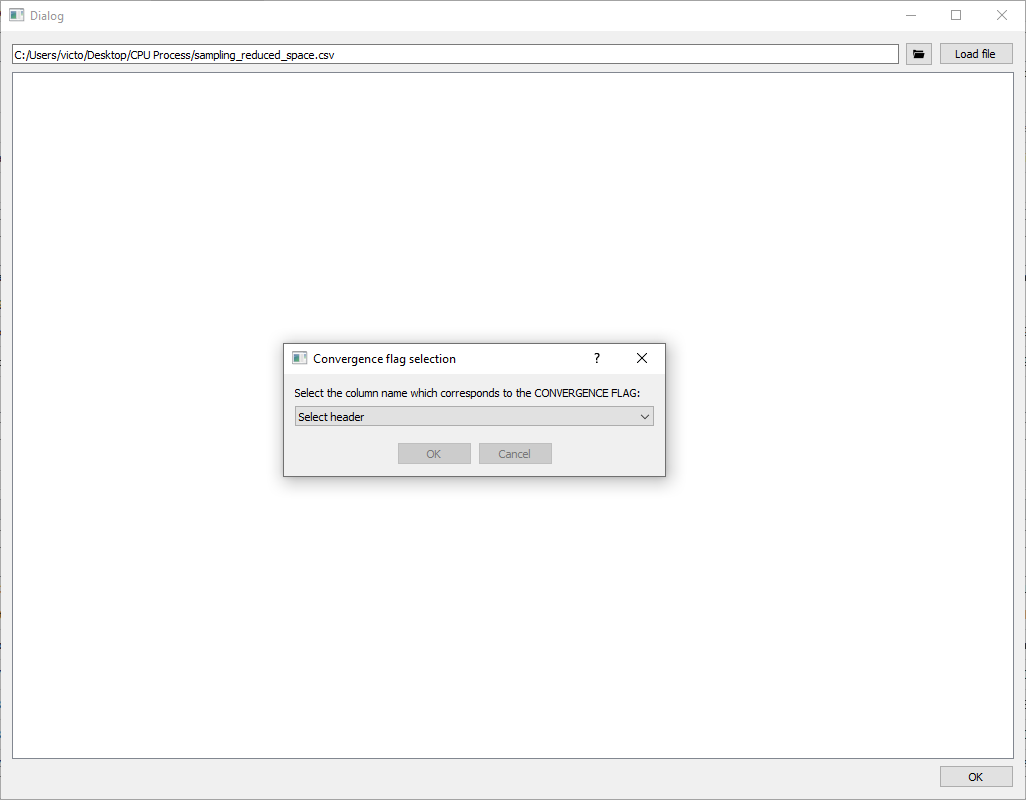
\includegraphics[width=1\textwidth]{csvload.PNG}}
\end{figure}

\begin{figure}[htb]
	\centering
	\caption{Associating each alias created in \mtc to each column
	of the *.csv data.}
	\label{fig:csvassociate}
    \makebox[1\textwidth]{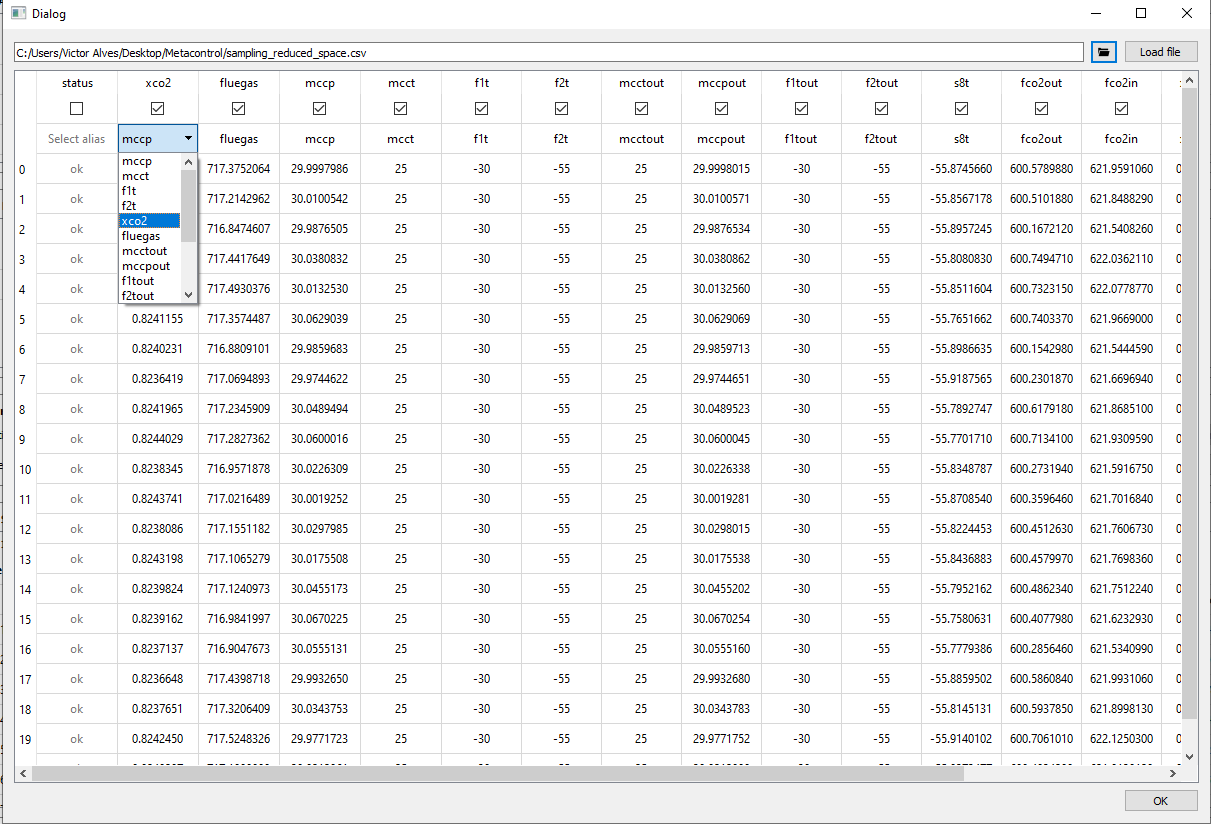
\includegraphics[width=1\textwidth]
    {csvassociate.PNG}}
\end{figure}

After importing the design of experiments from the external source (*.csv) 
and associating each variable created in \mtc with the data (as shown in 
\autoref{fig:csvassociate}), the user can go to ``Differential data'' tab, 
in order to generate the reduced space metamodel. Under the panel 
``Reduced space metamodel training'' the button ``Open training dialog'' 
allows the modification of the \kriging parameters, similarly as done 
previously in the step of generating the first metamodel to inspect the 
initial sampling.

\begin{figure}[htb]
	\centering
    \caption{``Differential data'' input screen: Reduced space model 
    training, Differentiation method, and gradient/hessian evaluation.}
	\label{fig:diffdatainput}
    \makebox[1\textwidth]{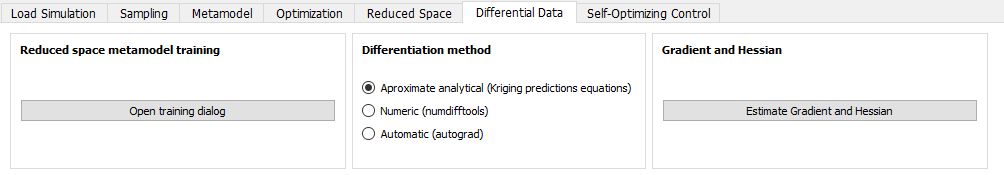
\includegraphics[width=1\textwidth]
    {diffdatainput.PNG}}
\end{figure}

The method of high-order data obtainment currently implemented in 
\mtc is based on the analytical expressions for the gradients 
and Hessian derived by \textcite{Lophaven2002} and \textcite{Alves2018}, 
respectively. In future releases of \mtc there will be two more methods 
of differentiation as secondary features. These will be based on numeric 
and automatic differentiation (\textit{numdifftools} and \textit{autograd} 
Python toolboxes, respectively), using the surrogate model as source of 
high-order data obtainment. However, it is strongly recommended the usage 
of the \kriging predictor analytical expressions to ensure results 
robustness, as stated before in \textcite{Alves2018}, and also stressed 
previously on this work.

After opening the training dialog (\autoref{fig:krigingredspace}) and 
configuring the reduced metamodel settings, the user can generate the 
metamodel, click on ``ok'', go back to the main screen and generate the 
estimation of the gradients and hessians necessary to carry on the \soc study.
These results are displayed on \autoref{fig:diffdataresults}.

\begin{figure}[htb]
	\centering
	\caption{Generating reduced space metamodel for CPU process: to avoid
    redundancy, the variables ``f1tout'', ``f2tout'', and ``mcctout'' were 
    not chosen in the reduced space problem since they correspond to the 
    decision variables that were found as active constraints. In general, 
    if the user decides to remove any variable previously set in the 
    problem, he must uncheck the undesired variable.}
	\label{fig:krigingredspace}
    \makebox[1.0\textwidth]{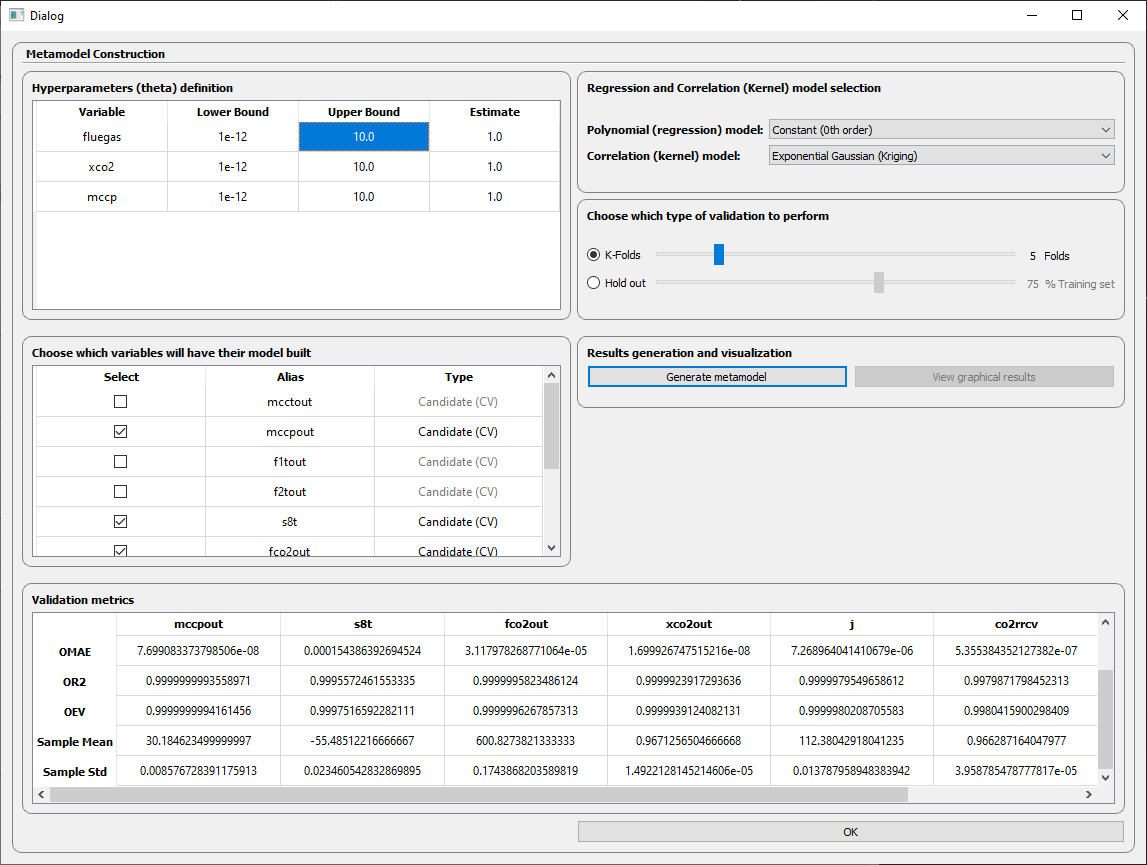
\includegraphics[width=1.0\textwidth]
    {krigingredspace.PNG}}
\end{figure}

\begin{figure}[htb]
	\centering
	\caption{Differential data estimated in \mtc}
	\label{fig:diffdataresults}
    \makebox[1.0\textwidth]{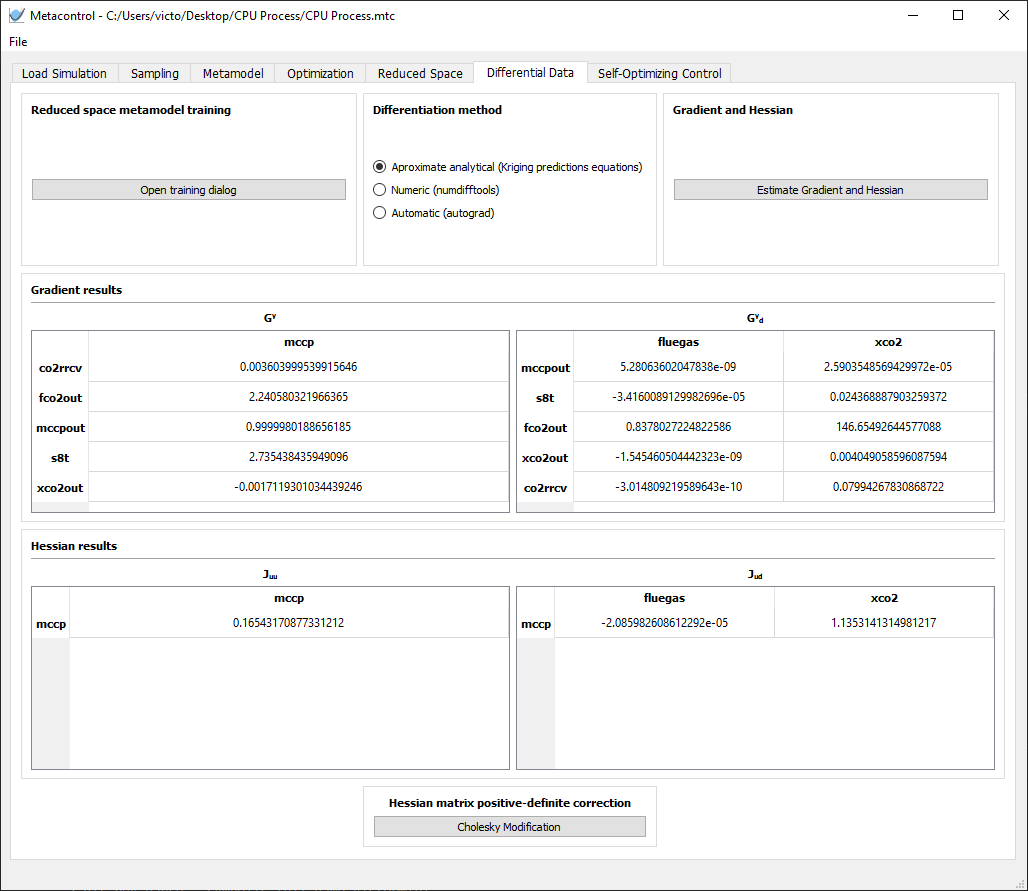
\includegraphics[width=1.0\textwidth]
    {gradresults.PNG}}
\end{figure}

In order to prove the effectiveness of the analytical expressions derived by 
\textcite{Lophaven2002} and already used in \textcite{Alves2018}, the 
gradients obtained using surrogate models in \mtc were compared against 
the ones generated in Aspen Plus (Equation-Oriented sensitivity mode). 
The process simulator does not provide the hessian of any function natively, 
and therefore $J_{uu}$ and $J_{ud}$  could not be compared. However, the 
excellent agreement between the values between the gradients found in both 
procedures can be considered as a sufficiently robust result.

\begin{table}[htb]
	\centering
	\caption{High-order data obtainment: \textit{Aspen Plus vs Metacontrol}}	
	\begin{tabular}{c c c}
		\hline
		 & $G^{y}$ & $G_{d}^y$ \\
		\hline
		\\
		\mtc & $
		\begin{bmatrix}
			\num{0.00360399953991565}\\ 
			\num{2.24058032196637}\\ 
			\num{0.999998018865619}\\ 
			\num{2.73543843594910}\\ 
			\num{-0.00171193010344392}
		\end{bmatrix}
		$ & 
		$
		\begin{bmatrix}
			\num{-3.01480921958964e-10} & \num{0.0799426783086872}\\ 
			\num{0.837802722482259}  & \num{146.654926445771}\\ 
			\num{5.28063602047838e-09}  & \num{2.59035485694300e-05}\\ 
			\num{-3.41600891299827e-05}  & \num{0.0243688879032594}\\ 
			\num{-1.54546050444232e-09} & \num{0.00404905859608759}
		\end{bmatrix}
		$ \\
		\\
		Aspen Plus & $
		\begin{bmatrix}
			\num{0.00360289000000000}\\ 
			\num{2.24032100000000}\\ 
			\num{1}\\ 
			\num{2.73303800000000}\\ 
			\num{-0.00171230000000000}
		\end{bmatrix}
		$ & 
		$
		\begin{bmatrix}
			\num{1.34722000000000e-07} & \num{0.0798491000000000}\\ 
			\num{0.837799400000000} & \num{146.612400000000}\\ 
			\num{0} & \num{0} \\ 
			\num{3.37970000000000e-15} & \num{0.0249510000000000}\\ 
			\num{1.69120000000000e-16} & \num{0.00404464000000000}
		\end{bmatrix}
		$ \\
		\\
		\hline
	\end{tabular}
	\label{tab:gradcomparison}
\end{table}

Through inspection of \autoref{tab:gradcomparison}, the reader can see how 
robust the results of the gradients obtained by the methodology proposed in 
the previous work from \textcite{Alves2018} and now are automated in \mtc. 
The matrix mean-squared error in \autoref{tab:msegradcpu} also corroborates 
this affirmation.

\begin{table}[htb]
	\centering
    \caption{Mean-squared error of high-order data obtaiment: 
    \textit{Aspen Plus vs Metacontrol} - CPU Process}	
	\begin{tabular}{l l l}
	\hline
	 & $G^{y}$ & $G_{d}^y$ \\ \hline
     Mean-squared error & \num{1.16586918414966e-06} & \num{1.8088e-04} \\ 
     \hline
	\end{tabular}
	\label{tab:msegradcpu}
\end{table}

After inspecting the gradients and hessians generated, the user can go to the 
``\soc'' tab, where the disturbances and measurement error magnitudes will be 
inserted. As stated previously in this case study, was considered a magnitude 
of $\pm5\%$ for the disturbances. For the $CO_{2}$ inlet composition, 
it was considered the absolute value, and for the flue gas flow rate, 
$\pm5\%$ of the nominal flow rate. Therefore, in \autoref{eq:wdcpu} :

\begin{equation}
	W_{d} = diag(0.05, 35.8595)
	\label{eq:wdcpu}
\end{equation}

In addition, for the measurement errors, it was considered $\pm0.5\celsius$ 
for temperature measurements, $0.01$ for pressure and flow measurements 
and $0.001$ for ratios ($CO_{2}$ recovery rate and product purity). 
These assumptions generated by \autoref{eq:wnycpu}:

\begin{equation}
	W_{n}^{y} = diag(0.001,0.01,0.01,0.5,0.001)
	\label{eq:wnycpu}
\end{equation}


The order for \Cref{eq:wdcpu,,eq:wnycpu} it is the same from the column order 
from \autoref{fig:diffdataresults}. \autoref{fig:socinput} shows the magnitude 
matrix data being inserted in \mtc.

\begin{figure}[htb]
	\centering
	\caption{Input screen in \mtc "\soc" tab - CPU Process}
	\label{fig:socinput}
    \makebox[1.0\textwidth]{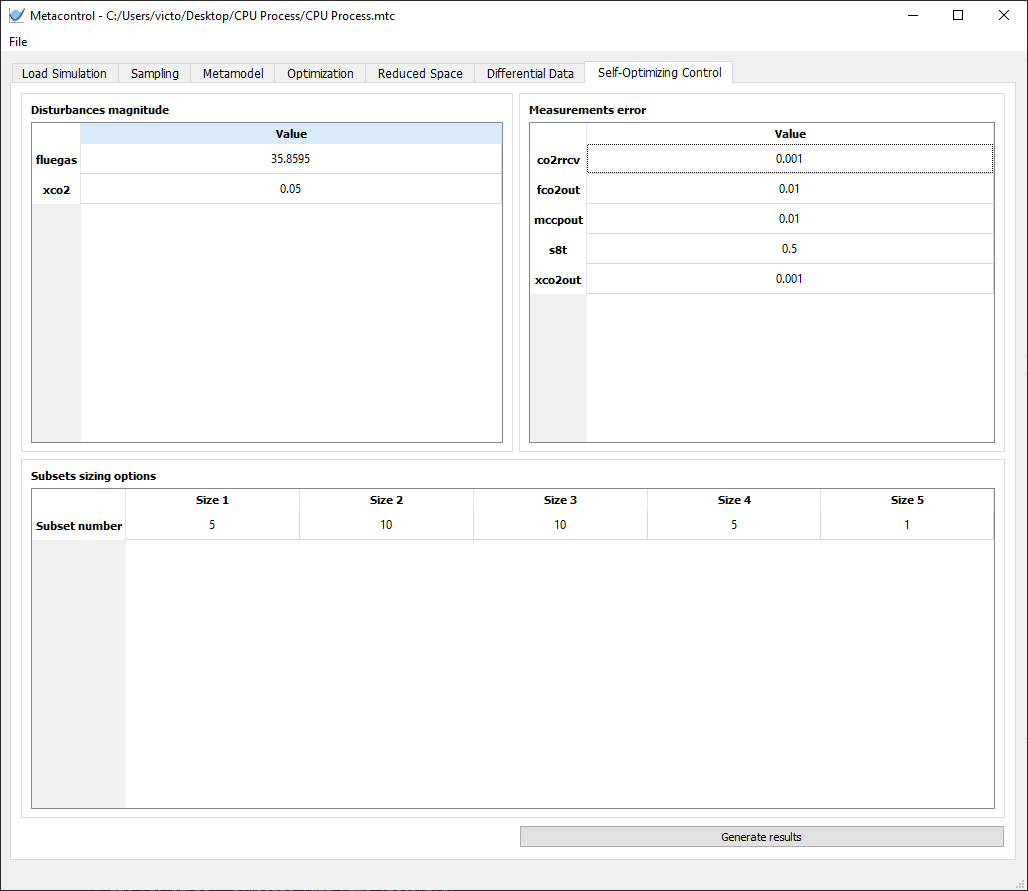
\includegraphics[width=1.0\textwidth]
    {soc_input.PNG}}
\end{figure}

Under the ``Subsets sizing options'' panel, by default the best control 
structure for each subset size is evaluated by \mtc, but the user can 
change how many subsets he wants to evaluate, until the maximum number 
for each subset size. 

After providing all the necessary inputs (magnitude matrices and number of best 
sets to be evaluated for each subset size), clicking in ``Generate results'' 
will show the $nth$ best \soc structures for each subset 
size, as can be seen for demonstration purposes in 
\Cref{fig:socresultss1,,fig:socresultss2}, the results for a single 
measurement policy, and for linear combinations using 2 measurements at a 
time. The user can also inspect the H matrix (that will be of ones and zeros 
for single measurements and a full matrix for linear combinations) and the 
optimal sensitivity matrix for each subset evaluated.

\begin{figure}[htb]
	\centering
	\caption{Best control structure in worst-case loss ascending order, for 
	subsets of size 1 (single measurement policy)}
	\label{fig:socresultss1}
    \makebox[1\textwidth]{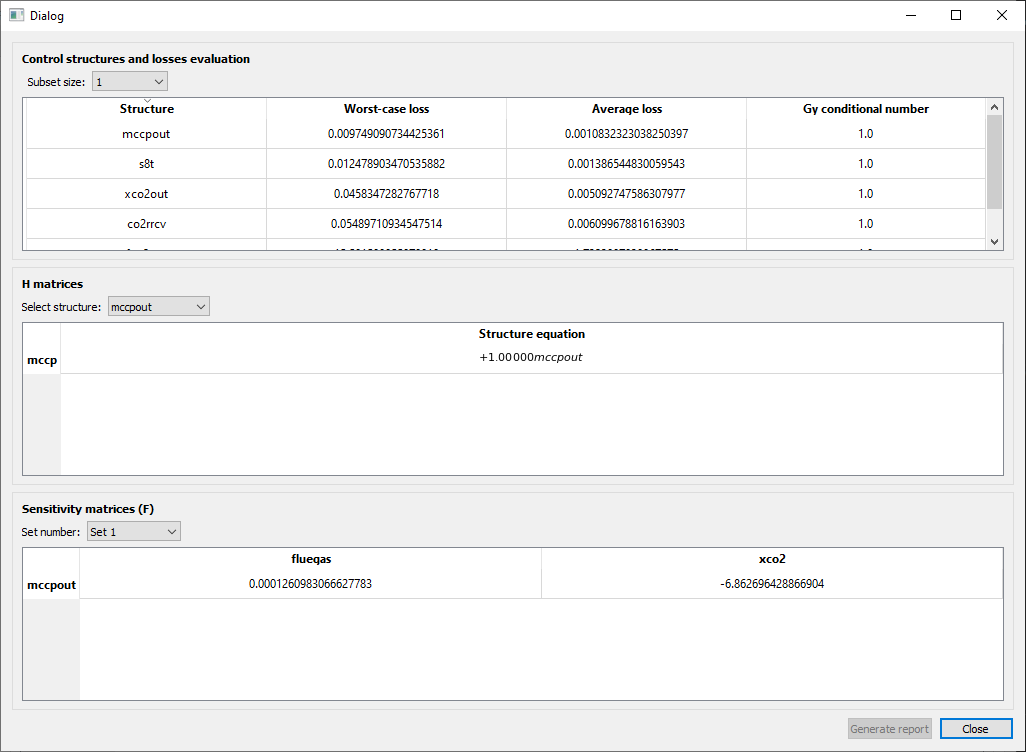
\includegraphics[width=1\textwidth]
    {soc_result_ss1.PNG}}
\end{figure}

\begin{figure}[htb]
	\centering
    \caption{Best control structure in worst-case loss ascending order, for 
    subsets of size 2 (linear combinations of measurements)}
	\label{fig:socresultss2}
    \makebox[1.0\textwidth]{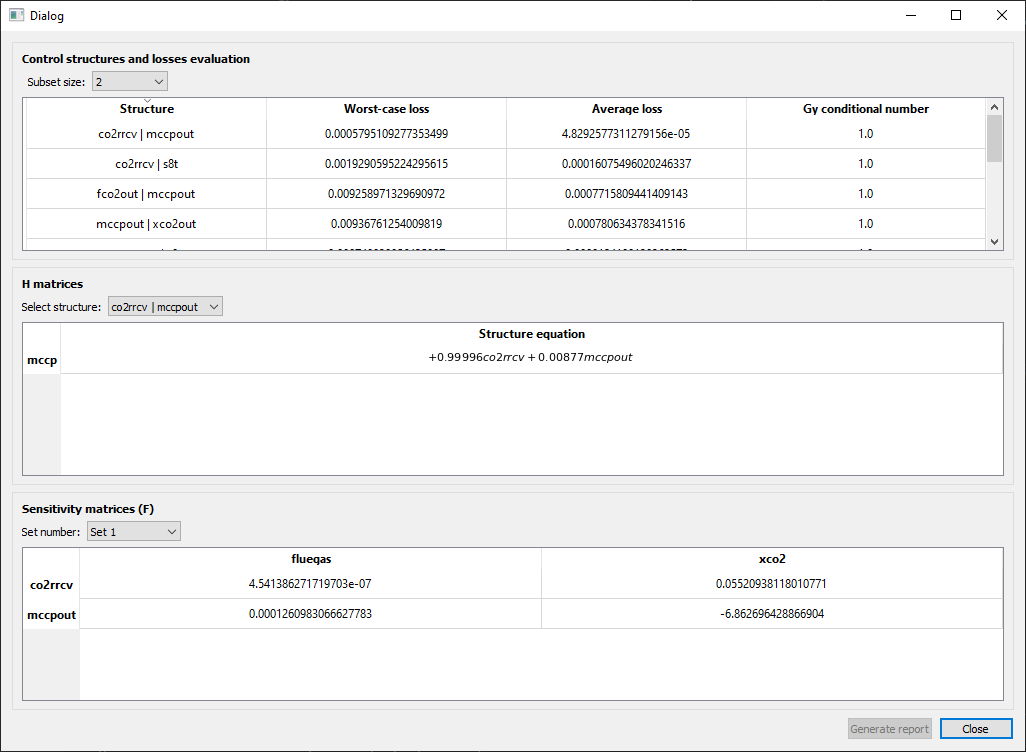
\includegraphics[width=1.0\textwidth]
    {soc_result_ss2.PNG}}
\end{figure}

For instance, considering a single measurement policy for the unconstrained 
degrees of freedom, \autoref{tab:bestcvscpu1} depicts the best CV candidates 
in worst-case loss ascending order. The best \soc variable for the considered 
case consists in the multi-stage compressor (MCC) outlet pressure. This 
result can be related to the previous finding \textcite{Liu2019}.

\begin{table}[htb]
	\centering
	\caption{Best \soc variables found by \mtc for a single measurement policy.}	
	\begin{tabular}{c c c}
	\hline
	CV Candidate  & Worst-Case  & Average-Case  \\ 
    \textit{alias} 
	& Loss $(kWh/tCO_{2})$ & Loss $(kWh/tCO_{2})$ \\ \hline
	mccpout & \num{0.009749090734425361} & \num{0.0010832323038250397} \\
	s8t & \num{0.012478903470535882} & \num{0.001386544830059543} \\
	xco2out & \num{0.0458347282767718} & \num{0.005092747586307977} \\
	co2rrcv & \num{0.05489710934547514} & \num{0.006099678816163903} \\
	fco2out & \num{15.591598055970818} & \num{1.7323997839967575} \\ \hline
    \end{tabular}
    {
        \nota{Description for the variables aliases present in 
        \autoref{tab:cvcandidateslist}.}
    }
	\label{tab:bestcvscpu1}
\end{table}

\FloatBarrier

\end{document}